\documentclass[aspectratio=169]{beamer}

\usetheme{Madrid}
\usecolortheme{dove}
\setbeamertemplate{navigation symbols}{}

\usepackage{tikz}
\usetikzlibrary{arrows.meta,positioning}
\usepackage{booktabs}

\title{Verifier-Driven Incident Response Agent Harness}
\subtitle{A narrow, demo-grade ops agent for deployment regressions}
\author{on-call-agent repository}
\date{\today}

\begin{document}

\begin{frame}
  \titlepage
\end{frame}

\begin{frame}{Problem Framing}
  \begin{itemize}
    \item Incident handling is not just ``call tools until the model sounds confident.''
    \item Real workflows need durable state, operator visibility, and explicit risk boundaries.
    \item Write actions such as rollback need approval and post-action verification against external
      runtime state.
    \item Recovery and handoff need structured artifacts, not only chat history.
  \end{itemize}

  \vspace{0.5em}
  \textbf{Design goal:} build the runtime spine that makes a narrow ops agent path inspectable,
  resumable, auditable, and verifier-backed.
\end{frame}

\begin{frame}{What This Project Is}
  \begin{columns}[T]
    \begin{column}{0.52\textwidth}
      \textbf{Repository today}
      \begin{itemize}
        \item verifier-driven incident-response runtime
        \item append-only transcripts and resumable checkpoints
        \item approval-gated bounded rollback path
        \item external outcome verification
        \item operator shell over the same runtime
      \end{itemize}
    \end{column}
    \begin{column}{0.44\textwidth}
      \textbf{Current live scope}
      \begin{itemize}
        \item one incident family: \texttt{deployment-regression}
        \item one mitigation: rollback to the known-good version
        \item shell modes:
          \texttt{manual}, \texttt{semi-auto}, \texttt{auto-safe}
        \item local demo target only
      \end{itemize}
    \end{column}
  \end{columns}

  \vspace{0.75em}
  \textbf{Not this project:} a mature ops platform, a coding agent, or broad autonomous
  remediation.
\end{frame}

\begin{frame}{Architecture Overview}
  \centering
  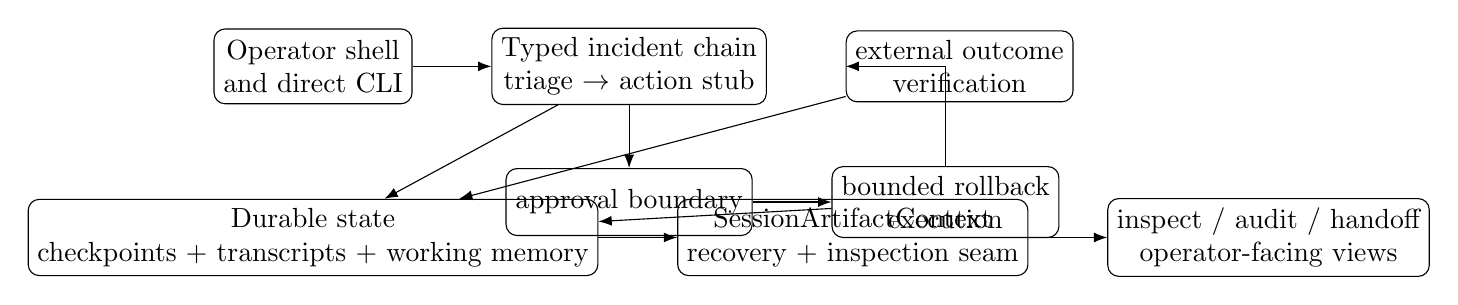
\begin{tikzpicture}[
    node distance=0.8cm and 1.0cm,
    box/.style={draw, rounded corners, align=center, minimum height=0.95cm, minimum width=2.5cm},
    smallbox/.style={draw, rounded corners, align=center, minimum height=0.85cm, minimum width=2.2cm},
    >=Latex
  ]
    \node[box] (shell) {Operator shell\\and direct CLI};
    \node[box, right=of shell] (chain) {Typed incident chain\\triage $\rightarrow$ action stub};
    \node[smallbox, below=of chain] (approval) {approval boundary};
    \node[smallbox, right=of approval] (rollback) {bounded rollback\\execution};
    \node[smallbox, right=of chain] (verify) {external outcome\\verification};

    \node[box, below=1.2cm of shell] (state) {Durable state\\checkpoints + transcripts + working memory};
    \node[box, right=of state] (context) {SessionArtifactContext\\recovery + inspection seam};
    \node[box, right=of context] (views) {inspect / audit / handoff\\operator-facing views};

    \draw[->] (shell) -- (chain);
    \draw[->] (chain) -- (approval);
    \draw[->] (approval) -- (rollback);
    \draw[->] (rollback) |- (verify);

    \draw[->] (chain) -- (state);
    \draw[->] (rollback) -- (state);
    \draw[->] (verify) -- (state);
    \draw[->] (state) -- (context);
    \draw[->] (context) -- (views);
  \end{tikzpicture}

  \vspace{0.6em}
  \small The shell is a thin product layer. It does not replace the runtime, approval seam, or
  durable-state model.
\end{frame}

\begin{frame}{Live Closed Loop}
  \centering
  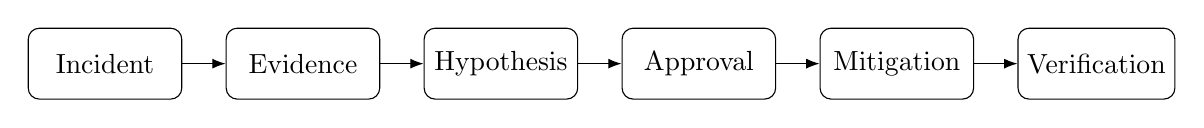
\begin{tikzpicture}[
    node distance=0.55cm,
    phase/.style={draw, rounded corners, align=center, minimum height=0.9cm, minimum width=1.95cm},
    >=Latex
  ]
    \node[phase] (incident) {Incident};
    \node[phase, right=of incident] (evidence) {Evidence};
    \node[phase, right=of evidence] (hypothesis) {Hypothesis};
    \node[phase, right=of hypothesis] (approval) {Approval};
    \node[phase, right=of approval] (mitigation) {Mitigation};
    \node[phase, right=of mitigation] (verification) {Verification};

    \draw[->] (incident) -- (evidence);
    \draw[->] (evidence) -- (hypothesis);
    \draw[->] (hypothesis) -- (approval);
    \draw[->] (approval) -- (mitigation);
    \draw[->] (mitigation) -- (verification);
  \end{tikzpicture}

  \vspace{0.9em}
  \begin{itemize}
    \item Evidence is collected from live \texttt{/deployment}, \texttt{/health}, and
      \texttt{/metrics} endpoints on the demo target.
    \item Mitigation is one bounded rollback candidate, not open-ended action planning.
    \item Verification re-probes external runtime state after the rollback.
  \end{itemize}
\end{frame}

\begin{frame}{Operator Shell And Autonomy Modes}
  \small
  \begin{tabular}{p{0.18\textwidth} p{0.26\textwidth} p{0.46\textwidth}}
    \toprule
    \textbf{Mode} & \textbf{Stops at} & \textbf{Behavior} \\
    \midrule
    \texttt{manual} & operator decision & analysis and inspection first; never auto-executes write actions \\
    \texttt{semi-auto} & approval boundary & drives the read-only chain to the rollback candidate, then waits for explicit approval \\
    \texttt{auto-safe} & fail-closed gate & only auto-runs the bounded rollback if the narrow policy, allowlist, evidence, version, and gap checks all pass \\
    \bottomrule
  \end{tabular}

  \vspace{0.8em}
  \begin{itemize}
    \item Mode is visible in shell status and durable in session checkpoints.
    \item If \texttt{auto-safe} cannot justify execution, the session degrades to
      \texttt{semi-auto} with a recorded reason.
    \item The shell adds operator UX, not hidden mutable state.
  \end{itemize}
\end{frame}

\begin{frame}{Why This Is Technically Credible}
  \begin{itemize}
    \item \textbf{Verifier-driven progression:} later phases only checkpoint after the matching
      verifier passes.
    \item \textbf{Approval boundary:} risky mutation remains explicit and inspectable.
    \item \textbf{External verification:} recovery is checked against live runtime endpoints, not
      only model output.
    \item \textbf{Durable recovery:} checkpoints, transcripts, and working memory can be rebuilt
      through \texttt{SessionArtifactContext}.
    \item \textbf{Auditability:} shell status, audit views, handoff export, and replay/eval all
      sit on the same durable artifacts.
  \end{itemize}
\end{frame}

\begin{frame}{What Is Intentionally Narrow}
  \begin{itemize}
    \item one incident family: recent deployment regression
    \item one bounded mitigation: rollback to a known-good version
    \item one demo target and one explicit allowlisted auto-safe scope
    \item operator shell over one runtime, not a second orchestration layer
    \item no claim of production readiness or broad autonomous remediation
  \end{itemize}

  \vspace{0.6em}
  \textbf{Why keep it narrow?} Because the point is to show harness discipline under real
  constraints before expanding breadth.
\end{frame}

\begin{frame}[fragile]{Demo / Usage Flow}
  \small
  \begin{verbatim}
oncall-agent run-demo-target --port 8001
oncall-agent shell

/sessions
/mode semi-auto
/new docs/examples/deployment_regression_payload.json
/status
/approve Rollback approved for the live demo target.
/verify
/handoff
  \end{verbatim}

  \begin{itemize}
    \item For a reviewer, this keeps the full incident lifecycle in one shell.
    \item \texttt{/why-not-auto} explains why \texttt{auto-safe} is or is not available.
    \item \texttt{/tail} gives a compact recent-activity view without leaving the session workspace.
  \end{itemize}
\end{frame}

\begin{frame}{Tradeoffs And Next Steps}
  \begin{columns}[T]
    \begin{column}{0.48\textwidth}
      \textbf{Current tradeoffs}
      \begin{itemize}
        \item narrow depth over broad feature count
        \item explicit seams over opaque autonomy
        \item local demo target over production integrations
        \item durable artifacts over chat-only memory
      \end{itemize}
    \end{column}
    \begin{column}{0.48\textwidth}
      \textbf{Reasonable next steps}
      \begin{itemize}
        \item add more scenario families only with the same verifier and approval discipline
        \item expand eval coverage for conservative and failure paths
        \item harden the operator shell around more replay and review workflows
      \end{itemize}
    \end{column}
  \end{columns}

  \vspace{0.8em}
  \textbf{Bottom line:} this is a narrow but real incident-response harness that demonstrates
  runtime engineering quality more than product breadth.
\end{frame}

\end{document}
